\documentclass[8pt]{beamer}
\usepackage{graphics}
\title{Auto-correlations of spins in East Model}
\author{Gang Huang}
\usetheme{Frankfurt}
\definecolor{mygreen}{rgb}{.3,.4,.12}
\usecolortheme[named=mygreen]{structure}

% Add page number
\setbeamertemplate{sidebar right}{}
\setbeamertemplate{footline}{%
	\hfill\usebeamertemplate***{navigation symbols}
	\hspace{1cm}\insertframenumber{}/\inserttotalframenumber}

\begin{document}
\maketitle

\section{1D East Model}
\begin{frame}
	\frametitle{East Model is an example of kinetically constrained Ising model.} 
	East model is a 1-D system of spins on lattice. For site $i$, $n_i =0$ or 1, with PBC. 
	
	No static interactions between spins. (\textbf{Jaeckle, Eisinger 1991; Eisinger, Jaeckle 1993; Faggionato, Martinelli, Roberto, and Toninelli 2012 })
	
	A given spin may only flip if the neighboring spin to the right is up, with an acceptance ratio $A$,
     \begin{alignat}{3}
       A = \left\{
       \begin{aligned}
	     e^{-\beta}, \text{ for } 01 \to 11 \\
         1, \text{ for } 11 \to 01.
       \end{aligned}
       \right
       .
     \end{alignat}
 East model shows glassy dynamics. (\textbf{Pitts and Andersen, 2001})
 %ie., its relaxation properties are similar to those of glass forming liquids and because some of them undergo ergodic–nonergodic transitions. 
 
 Define auto correlation function
      \begin{alignat}{3}
      C(t) = \frac{\langle\delta n_i(t)\delta n_i (0)\rangle}{\langle \delta n_i(0)^2 \rangle}.
 \end{alignat}
$\langle \cdots \rangle$: Average for the equilibrium state,

$n_i$: occupation number of site $i$.
\end{frame}

\begin{frame}
	\frametitle{Relation between $\beta$ and $c$}
	Denote $c = \langle n_i \rangle_{\text{eq}}$ (\textbf{Eisinger and Jaeckle, 1991}),
	\begin{alignat}{3}
		c= \frac{e^{-\beta}}{1+ e^{-\beta}} \Rightarrow \beta = \ln \frac{c}{1-c} \text{ for } c < 1/2.
	\end{alignat}
	(\textbf{Wu Jianlan, 2004, JPC})	
	\begin{alignat}{3}
		c = 0.10 \rightleftarrows \beta = 2.20 \nonumber\\
		c = 0.20 \rightleftarrows \beta = 1.39 \nonumber\\
		c = 0.30 \rightleftarrows \beta = 0.84 \nonumber\\
		c = 0.48 \rightleftarrows \beta =  0.05 
	\end{alignat}
\end{frame}

\begin{frame}
	\frametitle{MC Move Scheme for 1-dimensional East model}
	\begin{itemize}
        \item All sites simultaneously update in ONE step. Each step, record the configuration. (21-12-20)
        \item N randomly chosen sites update one by one. Every N updates, record the configuration. (22-1-10, \textbf{current version})
    \end{itemize}
\end{frame}

\section{Spin autocorrelation functions $C(t)$}
\begin{frame}
	\frametitle{$C(t)$ for 1-dimensional East model}
	\begin{figure}
		\centering
		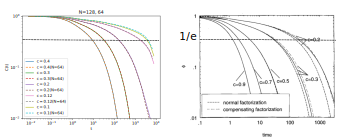
\includegraphics [width=1.1\textwidth] {./imag/corr_of_c_east_model.pdf}
		\setlength{\abovecaptionskip}{0pt}
		\caption{$C(t)$ from MC simulations  and from \textbf{Eisinger and Jaeckle (1993)}. PROBLEM: to speed up the program.}
	\end{figure}
\end{frame}

\begin{frame}
	\frametitle{Exact  $C(t)$ for 1-dimensional East model}
	\begin{figure}
		\centering
		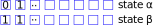
\includegraphics [width=0.7\textwidth] {./imag/exact_corr_of_c_east_model.pdf}
		\setlength{\abovecaptionskip}{0pt}
		\caption{Exact $C(t)$ (solid lines) from \textbf{numerical results} for finite chains (\textbf{Eisinger and Jaeckle, 1991)}.}
	\end{figure}
\end{frame}

\begin{frame}
	\frametitle{{\textcolor{blue}{$\beta$-dependence}} of $C(t)$ (semi-log plot)}
 \begin{figure}
	\centering
	\includegraphics [width=0.9\textwidth] {./imag/beta_dependence_of_corr_N128_step3000.pdf}
	\setlength{\abovecaptionskip}{0pt}
	\caption{{\textcolor{blue}{$t$-dependence}} and {\textcolor{blue}{$\beta$-dependence}} of $C(t)$}
\end{figure}
\end{frame}

\begin{frame}
	\frametitle{{\textcolor{blue}{$\beta$-dependence}} of relaxation time $\tau$}
	\begin{figure}
		\centering
		\includegraphics [width=0.7\textwidth] {./imag/relaxation_time_of_corr_on_beta_N128_step3000.pdf}
		\setlength{\abovecaptionskip}{0pt}
		\caption{{\textcolor{blue}{$\beta$-dependence}} of $C(t)$. $N=128$.}
	\end{figure}
\end{frame}

\begin{frame}
	\frametitle{{\textcolor{blue}{$c$-dependence}} of relaxation time $\tau$}
	\begin{figure}
		\centering
		\includegraphics [width=0.7\textwidth]
		{./imag/relaxation_time_of_corr_on_c_N128_step3000.pdf}
		\setlength{\abovecaptionskip}{0pt}
		\caption{{\textcolor{blue}{$c$-dependence}} of $C(t)$. $N=128$.}
	\end{figure}
\end{frame}

\section{Size effects}
\begin{frame}
	\frametitle{{\textcolor{blue}{$c$-dependence}} of $C(t)$.}
	\begin{figure}
		\centering
		\includegraphics [width=0.7\textwidth]
		{./imag/N_dependence_of_corr_beta2.00_step2400.pdf}
		\setlength{\abovecaptionskip}{0pt}
		\caption{{\textcolor{blue}{$N$-dependence}} of $C(t)$ is not obvious in these simulations.}
	\end{figure}
\end{frame}

\section{Conclusions}
\begin{frame}
	\frametitle{For $C(t)$:}
    %\begin{itemize}
    %	\item 
    %	%\item $\tau(\beta) \sim  \exp(\beta^2 \ln2)$ (\textbf{Sollich, Evans PRE 2003})
    %\end{itemize}	
\end{frame}

\section{Appendix}
\begin{frame}
	\frametitle{Concepts: Facilitating set}
	\begin{itemize}
		\item In each model, for each site $i$ there is a set of $f$ neighboring sites $S(i)$ s.t. the spin on site $i$ can flip only if all the spins on the sites $S(i)$ are up.
		\item \textbf{Facilitating set} $S(i)$ of site $i$ for the East model: spin $i+1$.
		
	\end{itemize}	
\end{frame}

\begin{frame}
	\frametitle{A simplifying case}
	Definitions:
	\begin{itemize}
		\item The \textbf{state} $\Gamma$ of a system of $N$ spins is specified by $n_1 ,\cdots,n_N$;
		\item The possible transitions of the system are those in which
		a single spin flips; 
		\item The flip rate for spin $i$ depends on the state of  spin $i+1$.
	\end{itemize}	
	Assumptions:
	\begin{itemize}
		\item The spins are statistically independent at equilibrium;
		%\item  All \textbf{sites} have the \textbf{same distribution function} for the occupation number, ie, $\forall i,  t=\infty,  p(n_i=0)= 1-e^{-\beta}, p(n_i =1) = e^{-\beta}$?
		\item  All \textbf{sites} have the \textbf{same distribution function} for the occupation number, ie, $\forall i,  t=\infty,  p(n_i=0)= 1-c, p(n_i =1) = c$;
		\item $\rho_0(\Gamma) = \prod_{i=1}^N p(n_i)$.
	\end{itemize}	
\end{frame}

\begin{frame}
	\frametitle{For $C(t)$:}
	\begin{itemize}
		\item $\phi(t) = \frac{\langle \delta n_i(t) \delta n_i(0)\rangle}{c(1-c)}$ (\textbf{Eisinger and Jaeckle, 1991}, where $\sigma_i =\pm 1$).
		\item   $C(t) = \frac{\langle\delta n_i(t)\delta n_i (0)\rangle}{\langle \delta n_i(0)^2 \rangle}$. What is the difference between $C(t)$ and $\phi(t)$ ? $n_i = \sigma_i = 0 \text{ or } 1$.
		\item $c=\langle n_i \rangle =0.9, 0.8$ (CHECK THIS PROBLEM! ?)
	\end{itemize}	
\end{frame}

\begin{frame}
	\frametitle{Theoretical object: to derive an equation of $C(t)$ (kinetic theory of $C(t)$)}
	In general,
	\begin{alignat}{3}
		\frac{dC(t)}{dt} + \omega C(t) + \omega^{-1} \int_0^t d\tau M^\text{irr}(t-\tau) \frac{dC(\tau)}{d\tau} = 0,
	\end{alignat}
where $\omega = k(0)$, $k(t) = -\frac{dC(t)}{dt}$, $M^\text{irr}$ is irreducible memory function.  (\textbf{Pitts, Andersen 2000})

In MCT, assume that
\begin{alignat}{3}
M^\text{irr}(t)=\sum_n a_n(c) [C(t)]^n. 
\end{alignat}
Some approximations:
\begin{itemize}
	\item  $M^\text{irr}_\text{K}(t) = c(1-c) [C(t)]^2$ (\textbf{Kawasaki1995})
	\item  $M^\text{irr}_\text{EJ}(t) = c(1-c) C(t) $ (\textbf{Eisinger and Jaeckle 1993} )
	\item diagrammatic representations of the irreducible memory function $\to$ obtained the irreducible memory kernel from a set of irreducible diagrams: $M^\text{irr} = c(1-c) C(t)$ for $(c< 0.5)$ (\textbf{Pitts, Young, Andersen, J. Chem. Phys. 2000, 113, 8671})
	 (\textbf{Pitts and Andersen, 2001})
	 \item A matrix formalism defined in the complete dynamic phase space (\textbf{Wu, Cao, J. Phys. Chem. B 2004, 108, 6796}).% (inspired by Pitts and Andersen).
\end{itemize}	
\end{frame}

\begin{frame}
	\frametitle{More about  $C(t)$: Detailed balance}
	Let the state $\alpha = (s_1,s_2,\cdots,s_N)$. In equilibrium,
	
	$ \frac{\partial P_\alpha(t)}{\partial t} = 0 \Rightarrow$ $P_\alpha(t) W_{\alpha\to \beta} = P_\beta(t) W_{\beta\to \alpha}$, where
	\begin{itemize}
		\item $P_\alpha(t)$ is the probability of the chain being in state $\alpha$.
		\item From detailed balance,$W_{a\to b} = e^{-\beta}$; $W_{b\to a} = 1 \Rightarrow$ 
		
		$P_b(t)/ P_a(t) = e^{-\beta}$ (see Figure).
	\end{itemize}	
	\begin{figure}
	\centering
	\includegraphics [width=0.4\textwidth]
	{./imag/detailed_balance_east_model.pdf}
	\setlength{\abovecaptionskip}{0pt}
	\caption{Two states of the 1-D finite East model with $N$ sites. }
    \end{figure}

\end{frame}

\begin{frame}
		\frametitle{More about  $C(t)$: Detailed balance condition (In general)}
We now restrict attention to systems for which there is a stationary distribution function
$\rho_0(\Gamma)$ s.t. the transition probabilities obey the DBC (\textbf{Pitts and Andersen, 2001}):
\begin{alignat}{3}
W(\Gamma',\Gamma) \rho_0(\Gamma) =W(\Gamma,\Gamma') \rho_0(\Gamma').
\end{alignat}

\end{frame}
\end{document}
